\documentclass[11pt,a4paper]{article}

\usepackage[margin=1in]{geometry}
\usepackage{amsmath, amssymb, mathtools}
\usepackage{fontspec}
\IfFontExistsTF{Times New Roman}
  {\setmainfont{Times New Roman}}
  {\setmainfont{Liberation Serif}}
\IfFontExistsTF{Arial}
  {\setsansfont{Arial}}
  {\setsansfont{Liberation Sans}}
\usepackage{newunicodechar}
\newunicodechar{≈}{\ensuremath{\approx}}
\newunicodechar{≤}{\ensuremath{\leq}}
\newunicodechar{≥}{\ensuremath{\geq}}
\newunicodechar{×}{\ensuremath{\times}}
\newunicodechar{−}{\ensuremath{-}}

\usepackage{xcolor}
\definecolor{headingcolor}{HTML}{1F4E79}
\definecolor{lightgray}{HTML}{666666}

\usepackage{setspace}
\onehalfspacing
\setlength{\parindent}{0pt}
\setlength{\parskip}{0.6em}

\usepackage{titlesec}
\titleformat{\section}
{\color{headingcolor}\sffamily\Large\bfseries}
{\thesection}{1em}{}
\titleformat{\subsection}
{\sffamily\large\bfseries}
{\thesubsection}{1em}{}

\usepackage{listings}
\lstset{
    basicstyle=\ttfamily\footnotesize,
    breaklines=true,
    columns=fullflexible,
    frame=single,
    framerule=0.4pt,
    showstringspaces=false,
    xleftmargin=0.4em,
    xrightmargin=0.4em,
    aboveskip=0.5em,
    belowskip=0.5em,
}

\usepackage{booktabs}
\usepackage{graphicx}
\usepackage{caption}
\captionsetup{font=small, labelfont=bf}

\newcommand{\courseheader}{
    \begin{center}
        {\sffamily\Large\bfseries CESE5040}\\[0.3em]
        {\sffamily High-Performance and AI Architectures}\\
        {\color{lightgray}2026 Q4}
    \end{center}
}

\newcommand{\Q}[1]{\subsection*{Question #1}}
\newcommand{\Qpart}[1]{\textbf{#1.}}

\begin{document}

\courseheader
\vspace{1em}

{\color{headingcolor}\sffamily\large\bfseries Student Information}

\textbf{Name:} Daniel Tyukov\\
\textbf{Student Number:} 5714699\\
\textbf{Lab:} Lab Assignment 4

{\color{headingcolor}\sffamily\large\bfseries Notes}

\begin{itemize}\setlength\itemsep{0.1em}
    \item Hardware: Intel Core Ultra 9 185H, CPU only. JAX 0.10.0, Flax 0.12.7, Optax 0.2.8, Python 3.12.
    \item Submitted: \texttt{L4\_Q4.py} and \texttt{L4\_Q6.py}. Q4.5 uses the supplied \texttt{mlp\_adv.py} architecture unchanged.
    \item Each accuracy is one run at the stated seed. Wall times cover the training loop only.
\end{itemize}

\vspace{0.5em}

\section*{\color{headingcolor}Lab Exercise 4}

% =========================================================================
\Q{4.1 - Backprop by hand and automatic differentiation}

\Qpart{1} Let $z^1_1 = w^1_{11}x_1 + w^1_{21}x_2 + b^1_1$, $z^1_2 = w^1_{12}x_1 + w^1_{22}x_2 + b^1_2$, and $z^2 = w^2_{11}h_1 + w^2_{21}h_2 + b^2_1$, with $h_i = \mathrm{ReLU}(z^1_i)$ and $y = \sigma(z^2)$. The loss is $\mathcal{L} = \tfrac{1}{2}(y - \hat{y})^2$, so $\partial \mathcal{L} / \partial y = (y - \hat{y})$ and $\partial y / \partial z^2 = y(1-y)$ from the sigmoid derivative.

For $w^2_{11}$ the chain runs $\mathcal{L} \to y \to z^2 \to w^2_{11}$:
\[
\frac{\partial \mathcal{L}}{\partial w^2_{11}}
= \frac{\partial \mathcal{L}}{\partial y}\,\frac{\partial y}{\partial z^2}\,\frac{\partial z^2}{\partial w^2_{11}}
= (y - \hat{y})\,y(1-y)\,h_1.
\]

For $w^1_{21}$ the chain goes one layer further back, through $h_1$:
\[
\frac{\partial \mathcal{L}}{\partial w^1_{21}}
= \frac{\partial \mathcal{L}}{\partial y}\,\frac{\partial y}{\partial z^2}\,\frac{\partial z^2}{\partial h_1}\,\frac{\partial h_1}{\partial z^1_1}\,\frac{\partial z^1_1}{\partial w^1_{21}}
= (y - \hat{y})\,y(1-y)\,w^2_{11}\,\mathbb{1}[z^1_1 > 0]\,x_2.
\]
The ReLU derivative is the indicator $\mathbb{1}[z^1_1 > 0]$, which is why dead ReLU units block any gradient signal from reaching $w^1_{21}$.

\Qpart{2} Autodiff frameworks record every elementary op of the forward pass along with its local Jacobian, then walk that graph to compute exact derivatives. Forward mode is cheap when there are few inputs and many outputs; reverse mode (backprop) is cheap in the opposite case, which is what training a scalar loss against millions of parameters demands. JAX, PyTorch, and TensorFlow trace the user's Python into an intermediate representation and apply the chain rule along the recorded edges. The user only writes the forward pass; gradients come back exactly and at near-forward cost, which is what makes deep networks trainable at all.

% =========================================================================
\Q{4.2 - MLP parameter count and CNN motivation}

\Qpart{1} With $I$ input neurons, $L$ hidden layers of width $H$, and $O$ outputs, the layer-by-layer count is:
\begin{itemize}\setlength\itemsep{0pt}
    \item Input to first hidden: $I H + H$ (weights plus bias).
    \item Between consecutive hidden layers: $H^2 + H$, repeated $L{-}1$ times.
    \item Last hidden to output: $H O + O$.
\end{itemize}
\[
\#\text{params} = IH + H + (L{-}1)(H^2 + H) + HO + O.
\]
For an MNIST-sized example with $I=784$, $L=2$, $H=512$, $O=10$ this gives about $670\text{k}$ parameters, which is already large for a simple toy.

\Qpart{2} Scaling this up is hopeless. A single 224$\times$224$\times$3 ImageNet image flattened into a $H=4096$ hidden layer already needs $\approx\!617$M parameters in one weight matrix. CNNs fix this with two priors: locality (each filter looks at a $k{\times}k$ window) and translation invariance (the same filter slides over the whole image). The parameter count drops from $H_{\text{in}} \cdot H_{\text{out}}$ to $k \cdot k \cdot C_{\text{in}} \cdot C_{\text{out}}$, which is independent of input resolution and several orders of magnitude smaller for typical $k = 3$ or $5$.

% =========================================================================
\Q{4.3 - Batching, learning rate, fit quality, loss vs accuracy}

\Qpart{1} Two reasons. Averaging the loss over a batch lowers the variance of the gradient estimate, so each step points more reliably than a single sample would. And hardware: GPUs need wide tensors to fill their tensor units, so a batch of 128 runs almost as fast as one image but does 128 times the useful work. A subtler effect is that very large batches lose the regularising noise of stochastic updates and settle into sharper minima that generalise worse. How the data is split also matters. A fixed order lets the model exploit it, so the convention is to reshuffle every epoch; with imbalanced classes a single-class batch will bias the gradient.

\Qpart{2} Too large and updates overshoot the minimum at every step; loss oscillates or diverges, often NaN within a few steps. Too small and the model moves in the right direction but never reaches a useful minimum in any reasonable budget. A scheduled rate gets both: start large to escape the random init, then decay (step, cosine, one-cycle) so the optimiser can settle. A short warmup at the very start helps when the early gradients are poorly conditioned.

\Qpart{3} Overfitting: training accuracy is high while test accuracy stalls or drops. The signature is a widening train-test gap (training loss still falling while validation loss climbs). Underfitting is the opposite: both train and test accuracy stay low because the model is too small or trained too short. Fixes are regularisation (L2, dropout), early stopping, or more data on the overfit side, and more capacity or more epochs on the underfit side.

\Qpart{4} The loss is a continuous, differentiable proxy for what we actually care about (top-1 accuracy here). It tracks the probability assigned to the correct class, so it reacts to the margin of every prediction; accuracy is binary per example. A model can keep driving cross-entropy down by becoming overconfident on examples it already gets right. That does nothing for accuracy and tends to coincide with overfitting: training loss keeps dropping while test accuracy plateaus. That is why the early-stopping signal of choice is validation accuracy or validation loss, not training loss.

% =========================================================================
\Q{4.4 - Simple MLP on MNIST (\texttt{L4\_Q4.py})}

\Qpart{1} \textit{Trained vs untrained accuracy at three seeds.}

\begin{table}[h]
\centering
\small
\begin{tabular}{rrrr}
\toprule
Seed & Untrained acc (\%) & Train acc (\%) & Test acc (\%) \\
\midrule
0  & 10.06 & 97.71 & 97.08 \\
10 & 9.41  & 97.74 & 97.10 \\
42 & 5.84  & 97.87 & 97.25 \\
\bottomrule
\end{tabular}
\caption{Per-sample SGD, $\alpha = 10^{-3}$, 10 epochs. Test accuracy spans only 0.17 pp across seeds.}
\end{table}

Untrained accuracy sits at chance ($\approx 10\%$ for ten classes), with seed 42 unlucky on the test set by random init. After ten epochs all three seeds land within 0.2 pp of each other. The seed moves the trajectory but not the final operating point, so for this small model trained accuracy is essentially seed-independent.

\Qpart{2} \textit{Effect of removing the [0,1] normalization.}

Dropping the \texttt{x/255} step at seed 10 collapsed test accuracy from 97.10\% to \textbf{11.34\%} (train 11.24\%), barely above chance. Raw pixels are about two orders of magnitude larger than the default LeCun-normal init expects, so the first pre-activations are huge, the gradient saturates, and the very first SGD step blows the parameters past any usable region. Normalising keeps activation statistics in the range the init was designed for.

\Qpart{3} \textit{Learning-rate sweep at \(\alpha \in \{10^{-1}, 10^{-4}, 10^{-7}\}\), seed 10.}

\begin{table}[h]
\centering
\small
\begin{tabular}{rrr}
\toprule
$\alpha$ & Train acc (\%) & Test acc (\%) \\
\midrule
$10^{-1}$ & 81.60 & 82.13 \\
$10^{-3}$ (baseline) & 97.74 & 97.10 \\
$10^{-4}$ & 92.14 & 92.55 \\
$10^{-7}$ & 11.39 & 11.17 \\
\bottomrule
\end{tabular}
\caption{Per-sample SGD, 10 epochs. The $10^{-3}$ row is reused from 4.4.1 for context.}
\end{table}

At $\alpha = 0.1$ updates are too aggressive for per-sample SGD; the model picks up the easy digits but never settles, ending 15 pp below baseline. At $\alpha = 10^{-4}$ the trajectory is healthy but ten epochs are not enough. At $\alpha = 10^{-7}$ the steps are so tiny that the parameters barely move from their random init.

\Qpart{4} \textit{Mini-batching for batch sizes 32, 64, 128, 256, 512.}

\begin{table}[h]
\centering
\small
\begin{tabular}{rrrr}
\toprule
Batch & Train acc (\%) & Test acc (\%) & Wall (s) \\
\midrule
32  & 89.39 & 89.93 & 4.5 \\
64  & 87.02 & 87.75 & 3.6 \\
128 & 83.34 & 84.28 & 2.4 \\
256 & 77.22 & 78.18 & 1.8 \\
512 & 67.84 & 68.43 & 1.4 \\
\bottomrule
\end{tabular}
\caption{$\alpha = 10^{-3}$, 10 epochs, seed 10. Compare against the per-sample baseline at the same $\alpha$ (97.10\% test, 85 s wall).}
\end{table}

\begin{figure}[h]
\centering
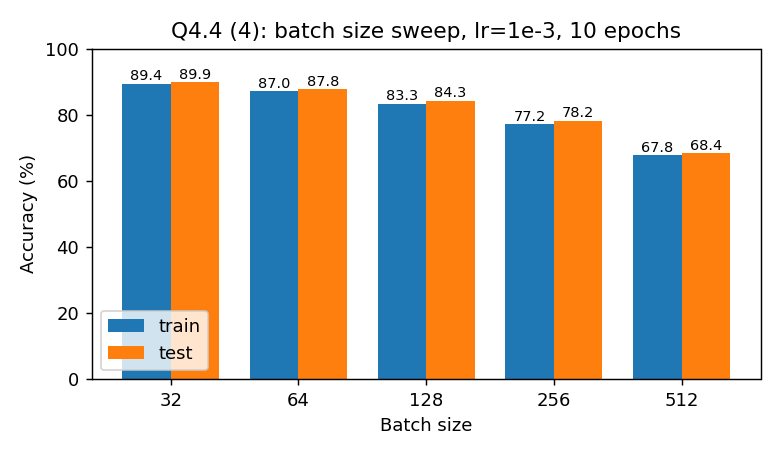
\includegraphics[width=0.75\linewidth]{../figures/q444_batch_sweep.png}
\caption{Test accuracy falls monotonically as batch size grows, at fixed $\alpha$.}
\end{figure}

Wall time drops because each batch is one JAX dispatch doing more work, and accuracy drops too because the number of weight updates per epoch shrinks from 60{,}000 (per-sample) to 117 (batch 512). With $\alpha$ pinned at $10^{-3}$ those few updates are not enough. This is the textbook setup for the linear scaling rule of learning rate to batch size, which 4.4.5 verifies.

\Qpart{5} \textit{Increasing the learning rate for batch size 64.}

\begin{table}[h]
\centering
\small
\begin{tabular}{rrr}
\toprule
$\alpha$ & Train acc (\%) & Test acc (\%) \\
\midrule
$10^{-3}$ (baseline) & 87.02 & 87.75 \\
$10^{-2}$ & 93.37 & 93.40 \\
$10^{-1}$ & 98.40 & 97.51 \\
$0.5$     & 99.35 & 97.65 \\
\bottomrule
\end{tabular}
\caption{Batch 64, seed 10, 10 epochs.}
\end{table}

\begin{figure}[h]
\centering
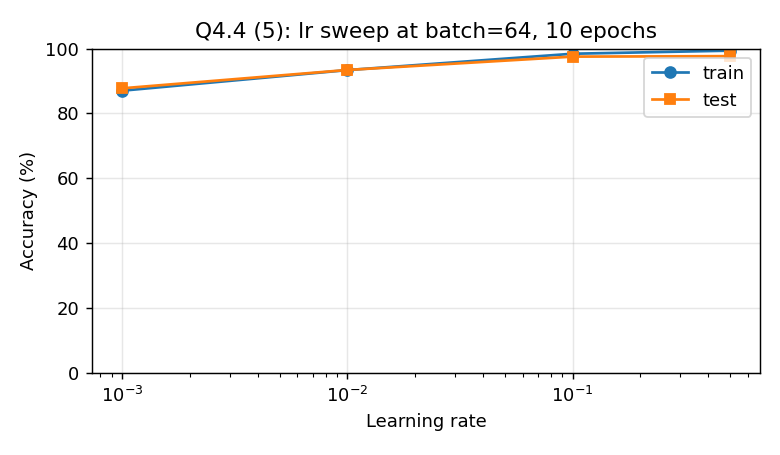
\includegraphics[width=0.75\linewidth]{../figures/q445_lr_sweep.png}
\caption{Bumping the learning rate recovers the accuracy lost by batching, exactly as the linear scaling rule predicts.}
\end{figure}

The same model that capped at 87\% with $\alpha = 10^{-3}$ reaches 97.5\% at $\alpha = 10^{-1}$, matching the per-sample baseline from 4.4.1. A batch gradient is the average of 64 sample gradients, so the per-step magnitude is roughly $1/64$ of the per-sample case and the rate has to be scaled up by a comparable factor. Beyond $\alpha \approx 0.1$ further gains shrink (train climbs, test stays put), which is the first whiff of overfitting.

\Qpart{6} \textit{Training set reduced to 1000 samples, 20 epochs, batch 64.}

\begin{table}[h]
\centering
\small
\begin{tabular}{rrrr}
\toprule
$\alpha$ & Train acc (\%) & Test acc (\%) & Gap (pp) \\
\midrule
$10^{-3}$ & 29.10 & 26.09 & 3.0 \\
$10^{-1}$ & 96.10 & 86.62 & 9.5 \\
\bottomrule
\end{tabular}
\caption{1000 samples, 20 epochs, batch 64, seed 10. Two regimes shown.}
\end{table}

With $\alpha = 10^{-3}$ at batch 64 there are only $1000 / 64 \cdot 20 \approx 312$ updates total, not enough to fit 1000 samples with a 101k-parameter model, so both numbers stay at the underfit floor. Switching to the working $\alpha = 10^{-1}$ from 4.4.5 fits the training set almost perfectly (96.1\%) while test accuracy lags ten points behind. That is the textbook overfit regime: plenty of capacity, too little data, no regularisation. On the full 60k set the same network generalises fine because more data acts as the regulariser.

% =========================================================================
\Q{4.5 - Regularised MLP (\texttt{mlp\_adv.py})}

\Qpart{1} \textit{What is dropout?} Dropout randomly zeroes a fraction $p$ of the activations during each training step and rescales the survivors by $1/(1-p)$ so the expected magnitude is preserved. At inference it is off and every unit participates. The effect is two-fold: neurons cannot co-adapt because any of them might be dropped, and the procedure is an implicit ensemble over the $2^n$ subnetworks defined by the dropout masks.

\Qpart{2} \textit{Is deeper / wider always better?} No. More layers and more width add capacity but also add parameters, memory, training time, and the risk of overfitting plus vanishing or exploding gradients (especially without residual connections or careful init). A 512-512 MLP already saturates MNIST; a 4096-4096-4096 stack would learn nothing the smaller model misses and just train slower. Depth pays off when the data has compositional structure, which is more true of images, audio and language than of MNIST digits.

\Qpart{3} \textit{AdamW and weight decay.} Adam combines momentum (first moment of the gradient) with per-parameter step normalisation (second moment), so each parameter takes a step adapted to its own gradient scale. AdamW is a small fix on top. Vanilla Adam folds an L2 penalty into the gradient before the moment normalisation, which ties the effective decay to the gradient magnitude and breaks the regularisation. AdamW decouples the decay and applies it directly to the parameters at update time, so the decay coefficient behaves as a clean shrinkage term. Its role matches L2: pull weights toward zero, keep them small, discourage overfitting.

\Qpart{4} \textit{Three-seed accuracy on \texttt{mlp\_adv.py}, 10 epochs.}

\begin{table}[h]
\centering
\small
\begin{tabular}{rrrr}
\toprule
Seed & Untrained acc (\%) & Train acc (\%) & Test acc (\%) \\
\midrule
0  & 6.65 & 99.40 & 97.96 \\
10 & 8.78 & 99.38 & 98.12 \\
42 & 9.47 & 99.56 & 98.24 \\
\bottomrule
\end{tabular}
\caption{\texttt{mlp\_adv.py} architecture (Dense 512, Dropout 0.3, Dense 512, Dropout 0.3, Dense 10), AdamW with $\alpha = 10^{-3}$, weight decay $10^{-4}$, batch 128, 10 epochs. Roughly 670{,}000 trainable parameters.}
\end{table}

Test accuracy of 97.96-98.24\% across seeds sits about a percentage point above the plain \texttt{mlp.py} baseline (97.08-97.25\%), with a train-test gap of about 1.3 pp. Three changes pull the same way: wider 512-512 hidden layers fit better than 128 units, AdamW converges faster than vanilla SGD because each parameter's step is rescaled by its own gradient variance, and dropout keeps the extra capacity from turning into extra overfitting.

% =========================================================================
\Q{4.6 - LeNet-5 (\texttt{L4\_Q6.py})}

\Qpart{1} \textit{Parameter count.} The LeNet-5 architecture from the assignment figure has the following parameter breakdown:

\begin{table}[h]
\centering
\small
\begin{tabular}{lrl}
\toprule
Layer & Params & Calculation \\
\midrule
C1 (Conv 1$\to$6, 5$\times$5)         & 156    & $5\cdot 5\cdot 1\cdot 6 + 6$ \\
S2 (AvgPool 2$\times$2)              & 0      & no parameters \\
C3 (Conv 6$\to$16, 5$\times$5)         & 2{,}416 & $5\cdot 5\cdot 6\cdot 16 + 16$ \\
S4 (AvgPool 2$\times$2)              & 0      & no parameters \\
F5 (Dense 400$\to$120)              & 48{,}120 & $400\cdot 120 + 120$ \\
F6 (Dense 120$\to$84)               & 10{,}164 & $120\cdot 84 + 84$ \\
Out (Dense 84$\to$10)               & 850     & $84\cdot 10 + 10$ \\
\midrule
\textbf{Total}                      & \textbf{61{,}706} & \\
\bottomrule
\end{tabular}
\caption{LeNet-5 parameter breakdown. Almost 80\% of the parameters live in F5 alone.}
\end{table}

The two conv stages together hold only $\approx$2.6k parameters even though they do most of the feature extraction; the dense layers carry the rest. That is already an order of magnitude smaller than the 670k of a 512-512 MLP.

\Qpart{2} \textit{Implementation notes.} Built with \texttt{flax.linen}. C1 uses \texttt{SAME} padding so the first feature map stays $28\times 28$ (the original LeNet padded the input to $32\times 32$; using SAME on the conv is the modern equivalent). C3 uses VALID padding to get $10\times 10$. Both pools are $2\times 2$ stride 2. All conv and dense layers use \texttt{tanh}. Optimiser is AdamW, batch 128.

\Qpart{3} \textit{Three-seed run at the default hyper-parameters, then a 3$\times$3 LR / weight-decay sweep at seed 10. All runs 10 epochs, batch 128.}

\begin{table}[h]
\centering
\small
\begin{tabular}{rrrr}
\toprule
Seed & Untrained acc (\%) & Train acc (\%) & Test acc (\%) \\
\midrule
0  & 6.45 & 99.32 & 98.40 \\
10 & 9.88 & 99.37 & 98.27 \\
42 & 7.89 & 99.37 & 98.48 \\
\bottomrule
\end{tabular}
\caption{LeNet-5, AdamW with $\alpha = 10^{-3}$, $\lambda_{\text{wd}} = 10^{-4}$. Test accuracy spans 0.21 pp across seeds.}
\end{table}

\begin{table}[h]
\centering
\small
\begin{tabular}{rrrr}
\toprule
$\alpha$ & $\lambda_{\text{wd}} = 0$ & $\lambda_{\text{wd}} = 10^{-4}$ & $\lambda_{\text{wd}} = 10^{-3}$ \\
\midrule
$10^{-2}$ & 96.49 & 96.71 & 97.31 \\
$10^{-3}$ & 98.27 & 98.27 & 98.25 \\
$10^{-4}$ & 96.75 & 96.75 & 96.75 \\
\bottomrule
\end{tabular}
\caption{Test accuracy from the LR $\times$ weight-decay sweep, seed 10, 10 epochs.}
\end{table}

\begin{figure}[h]
\centering
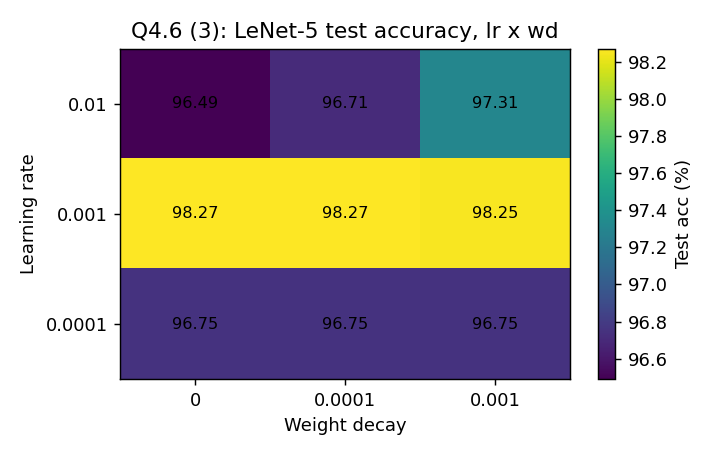
\includegraphics[width=0.7\linewidth]{../figures/q463_lr_wd_heatmap.png}
\caption{LeNet-5 test accuracy as a function of learning rate and weight decay. The $\alpha = 10^{-3}$ row is uniformly the best regardless of weight decay.}
\end{figure}

Learning rate carries almost all the signal. $\alpha = 10^{-3}$ is the sweet spot at 98.27\%, $\alpha = 10^{-2}$ overshoots (the optimiser oscillates near the minimum), $\alpha = 10^{-4}$ undertrains in 10 epochs. Weight decay barely moves the needle at $\alpha = 10^{-3}$ and is invisible at $\alpha = 10^{-4}$, because AdamW's per-step shrinkage is proportional to $\alpha \cdot \lambda_{\text{wd}}$, so a small rate shrinks the decay scale too. The one place decay pays off is at $\alpha = 10^{-2}$, where stronger regularisation damps the oscillation and recovers about 0.8 pp.

\Qpart{4} \textit{LeNet-5 vs MLP comparison.}

\begin{table}[h]
\centering
\small
\begin{tabular}{lrrr}
\toprule
Model & Params & Best test acc (\%) & Configuration \\
\midrule
\texttt{mlp.py} (per-sample SGD)       & $\approx$101k & 97.25 & seed 42, $\alpha = 10^{-3}$, 10 epochs \\
\texttt{mlp.py} (batched, scaled LR)   & $\approx$101k & 97.65 & seed 10, $\alpha = 0.5$, batch 64 \\
\texttt{mlp\_adv.py} (Dropout + AdamW) & $\approx$670k & 98.24 & seed 42, $\alpha = 10^{-3}$, $\lambda_{\text{wd}} = 10^{-4}$ \\
LeNet-5                                & 61.7k & \textbf{98.48} & seed 42, same hyper-params as above \\
\bottomrule
\end{tabular}
\caption{Best test accuracy reached by each model on this lab. LeNet-5 wins despite having an order of magnitude fewer parameters than the deepest MLP.}
\end{table}

LeNet-5 has roughly ten times fewer parameters than the wide MLP (61.7k vs 670k) and still generalises a few tenths of a percentage point better. The reason is inductive bias. A conv layer encodes two priors: pixels close together are more related than pixels far apart, and the same feature can appear anywhere in the image. Both hold for digits, so the parameter budget goes into filters that match the input rather than into independent pixel-to-hidden-unit edges. The MLP has neither prior; most of its 670k parameters re-discover correlations a convolution captures for free. On MNIST the wastage costs only a few tenths of a percentage point. On richer data like CIFAR-10 or ImageNet the same inductive bias is the difference between a model that trains and one that does not.

% =========================================================================

\vspace{1em}

% LLM Disclosure
{\color{headingcolor}\sffamily\large\bfseries LLM Usage Disclosure}

\vspace{0.3em}

I used Claude Code on this lab for:
\begin{itemize}
    \item Cross-checking the Flax conv / pool API and the AdamW signature in Optax against the documentation while implementing LeNet-5.
    \item Editing the report (tightening phrasing, trimming filler).
\end{itemize}

\end{document}
